\documentclass{homeworg}
\usepackage{amsmath}
\usepackage{xcolor}

\title{Travail 7 - Diagramme de Karnaugh}
\author{Wats Raphaël}

\begin{document}
\maketitle

\section{La table de vérité}
\begin{center}
    \LARGE
    \begin{tabular}{|l|c|r|r|r|}
        \hline
            A & B & C & D & Y\\
        \hline
            0 & 0 & 0 & 0 & 1\\
            0 & 0 & 0 & 1 & 1\\
            0 & 0 & 1 & 0 & 0\\
            0 & 0 & 1 & 1 & 0\\
            0 & 1 & 0 & 0 & 0\\
            0 & 1 & 0 & 1 & 0\\
            0 & 1 & 1 & 0 & 1\\
            0 & 1 & 1 & 1 & x\\
            1 & 0 & 0 & 0 & x\\
            1 & 0 & 0 & 1 & x\\
            1 & 0 & 1 & 0 & 0\\
            1 & 0 & 1 & 1 & 1\\
            1 & 1 & 0 & 0 & 0\\
            1 & 1 & 0 & 1 & 0\\
            1 & 1 & 1 & 0 & 1\\
            1 & 1 & 1 & 1 & x\\
        \hline
    \end{tabular}
\end{center}
\newpage

\section{Le diagramme de Karnaugh}
\begin{center}
    \Huge
    \begin{tabular}{|c|c|c|c|c|}
        \hline
        CD / AB & 00 & 01 & 11 & 10\\
        \hline
        00 & \color{red} 1 & 0 & 0 & \color{red} x\\
        01 & \color{red} 1 & 0 & 0 & \color{red} x \color{green} x\\
        11 & 0 & \color{blue} x & \color{blue} x & \color{green} 1\\
        10 & 0 & \color{blue} 1 & \color{blue} 1 & 0\\
        \hline
    \end{tabular}
\end{center}

\section{La fonction logique optimée}
\begin{center}
    \Huge
    $
    \color{red} \overline{B} \overline{C} +
    \color{blue} BC +
    \color{green} A \overline{B} D
    $
\end{center}

\section{Le schéma du circuit}
\begin{center}
    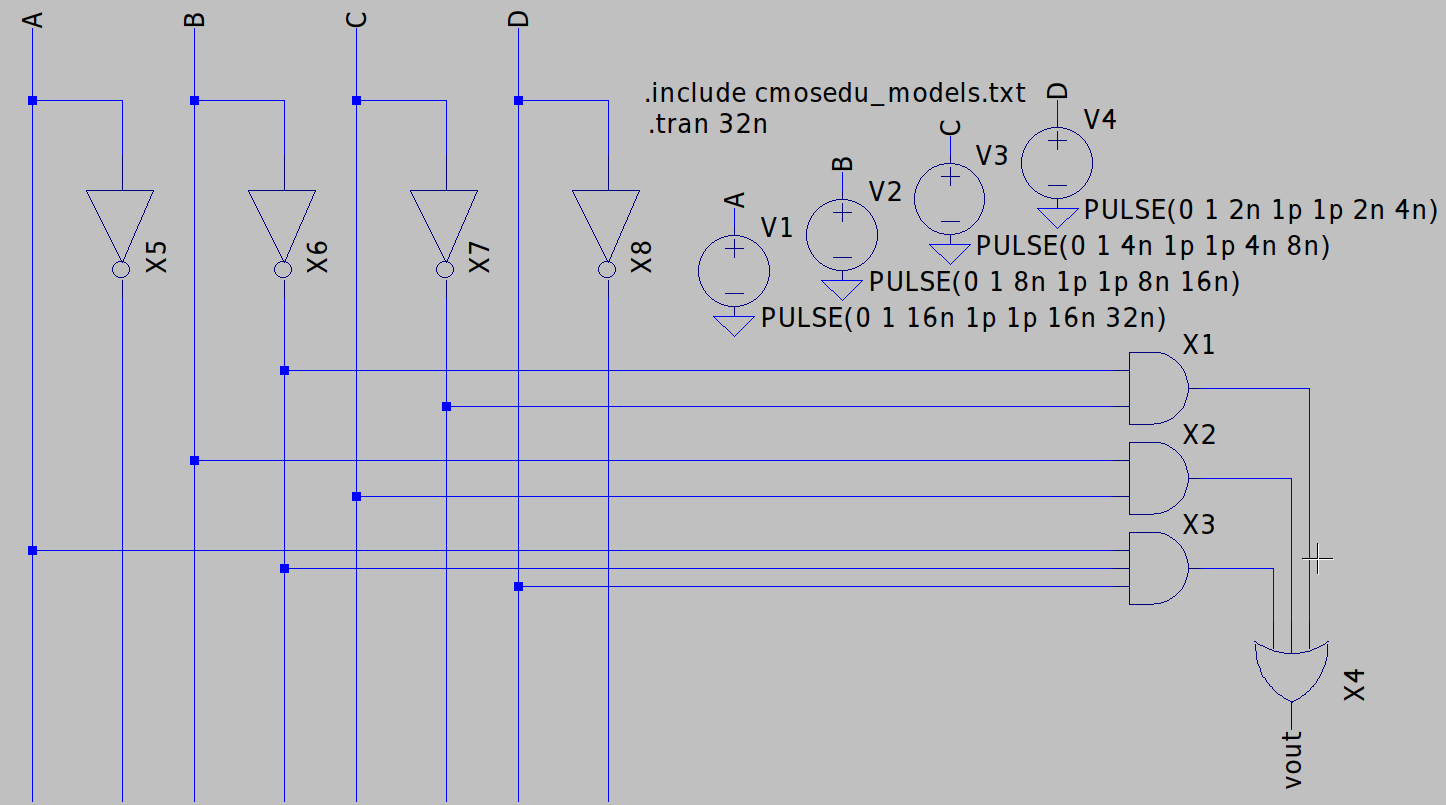
\includegraphics[scale=0.41]{circuit.png}
\end{center}
\newpage

\section{La simulation en parcourant les 16 états de la table de vérité}
\begin{center}
    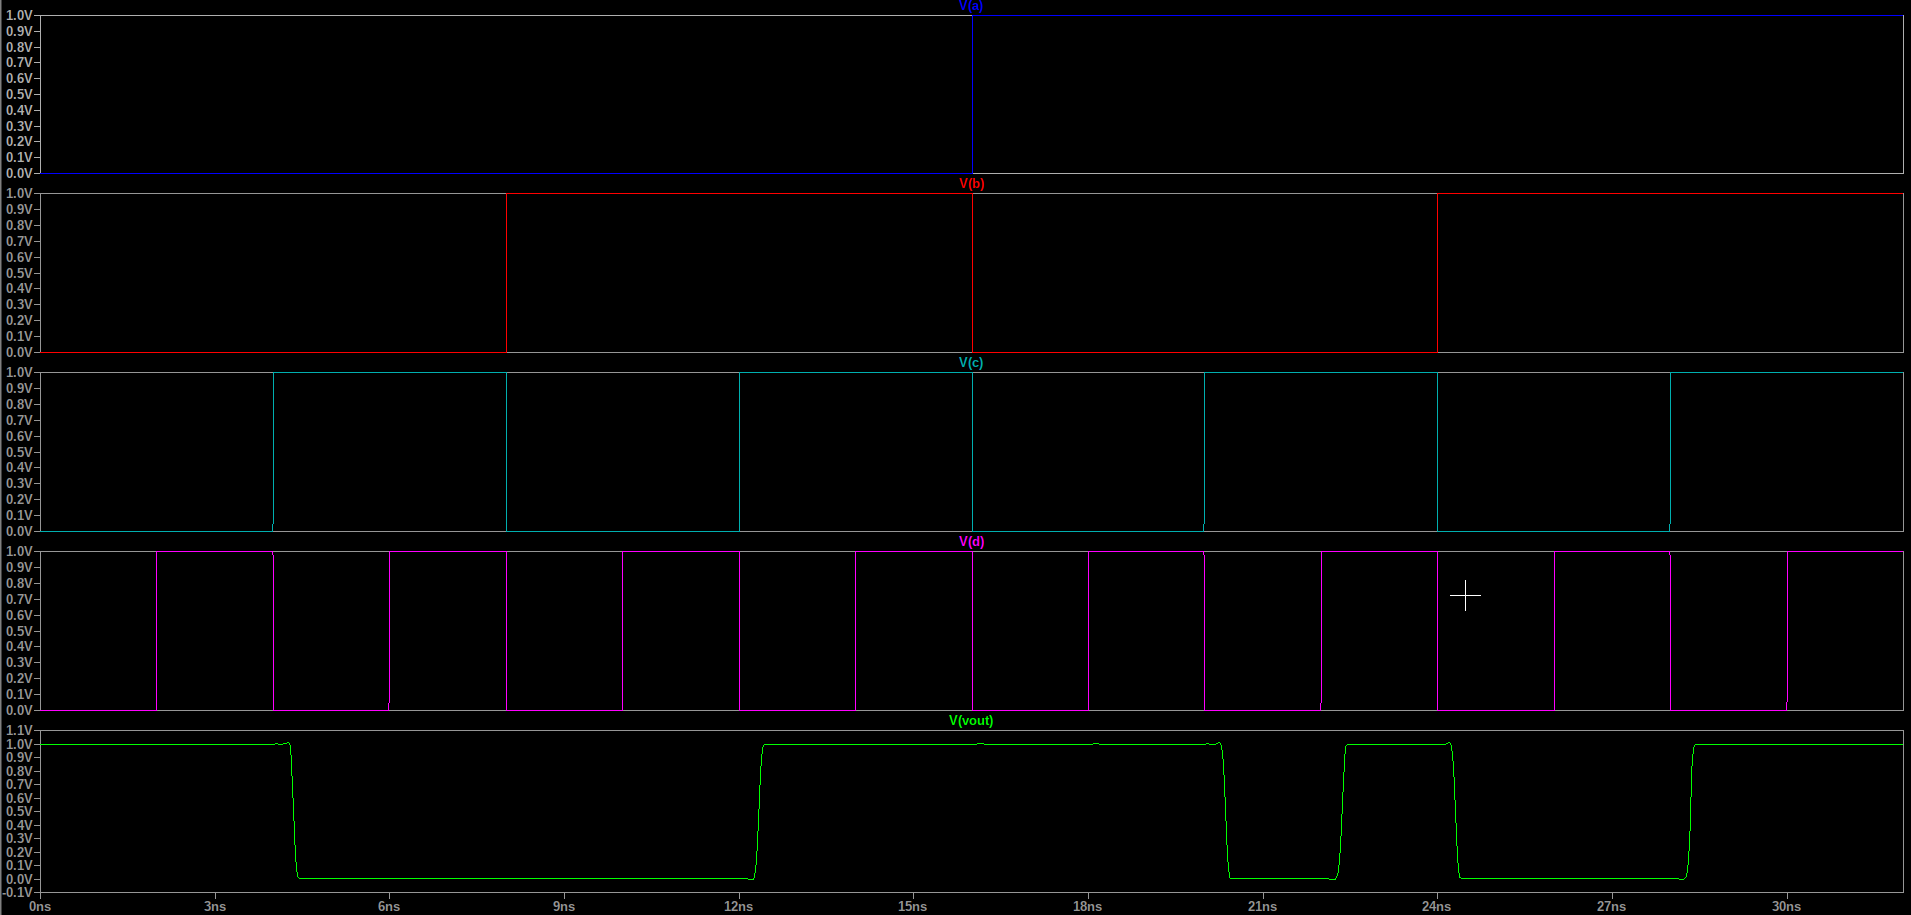
\includegraphics[scale=0.31]{truth.png}
\end{center}
\section{Les temps de contamination et de propagation}
Le temps de contamination correspond au temps de variation le plus court de l'output après la variation d'un de ses inputs.
On peut le trouver en observant le graphe d'une simulation transitoire du circuit opposant l'output avec l'input ayant le chemin le plus court vers l'output.
\begin{center}
    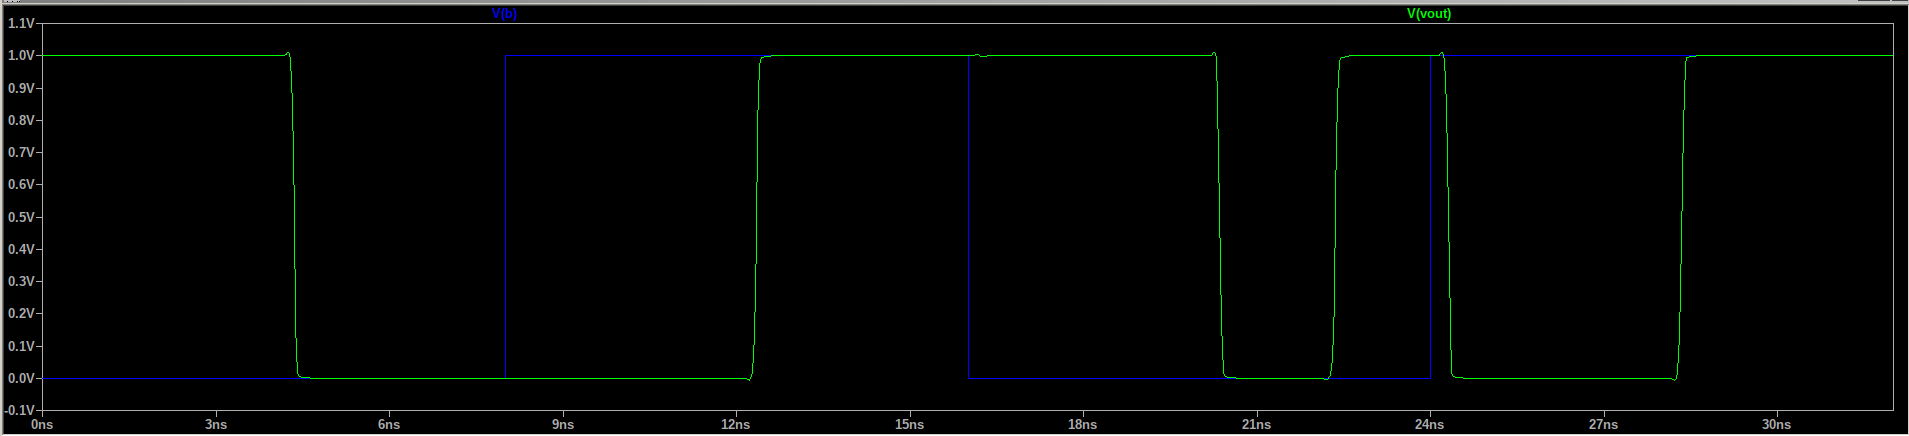
\includegraphics[scale=0.31]{timing_a.png}
\end{center}
A $24n$ secondes en zoomant on peut observer un délai d'à peu près $0.4n$ secondes.
\begin{center}
    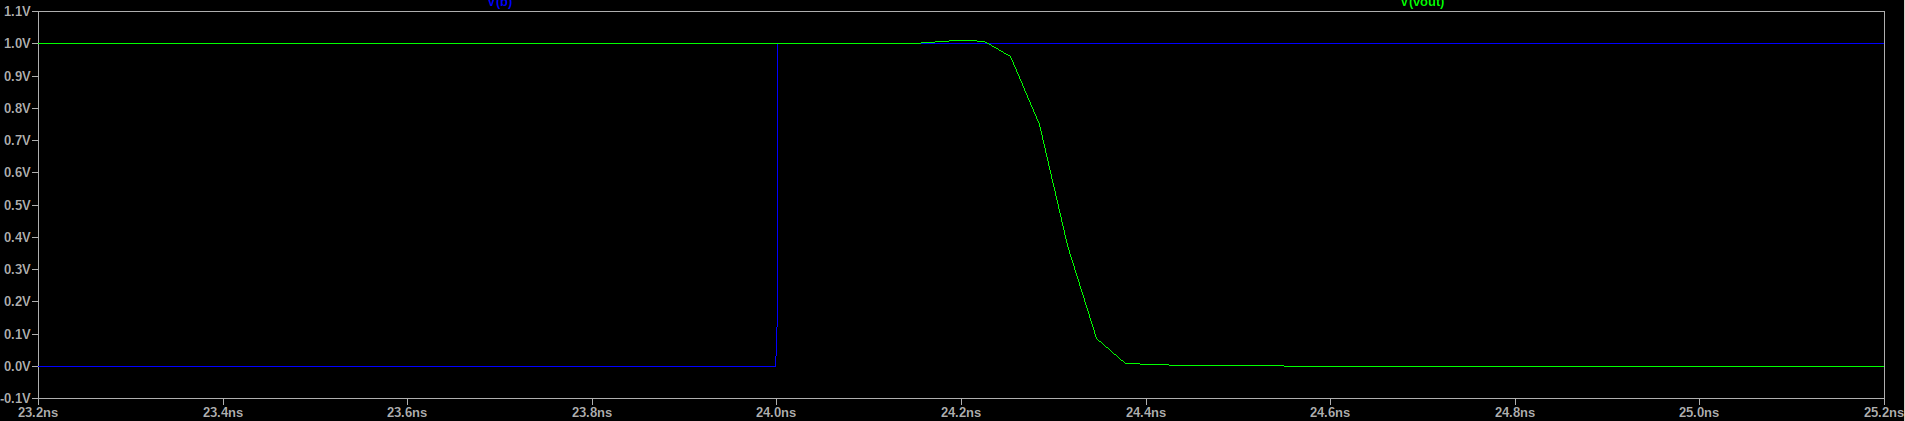
\includegraphics[scale=0.31]{timing_b.png}
\end{center}
Le temps de propagation correspond au temps de variation le plus long de l'output après la variation d'un de ses inputs.
On peut le trouver en observant le graphe d'une simulation transitoire du circuit opposant l'output avec l'input ayant le chemin le plus long vers l'output.

Grâce à la configuration du circuit, le chemin le plus court est égale au chemin le long donc le temps de propagation est égale au temps de contamination c'est à dire $0.4n$ secondes.
\newpage

\section{Conclusion}
Les résultats obtenu sont en adéquation avec ceux obtenu lors des simulations LTspice XVII.
\begin{itemize}
    \item Un diagramme de Karnaugh permet d'appliquer un algorithme efficace pour déterminer une fonction logique optimale.
    \item La configuration du circuit est efficace pour éviter les glitches dû aux temps de propagation et de contamination.
    \item Lorsque l'on design des circuits digitaux CMOS il faut faire attention aux glitches dû au temps de propagation et de contamination.
\end{itemize}

\end{document}
